\documentclass[10pt,a4paper]{article}
\usepackage[latin1]{inputenc}
\usepackage{amsmath}
\usepackage{amsfonts}
\usepackage{amssymb}
\usepackage{booktabs}
\usepackage{graphicx}
\usepackage{listings}
\usepackage{subfigure}
\usepackage{float}
\usepackage{hyperref}

\title{Local Structure - assignment 4}
\author{Jayke Meijer (6049885), Richard Torenvliet (6138861)}

\begin{document}
\maketitle

\section{Introduction}

In this exercise we implement a few exercises with the goal to learn 
the effect of Gaussian derivatives as part of a convolution. Using this,
we will finally implement the `Canny Edge Detector'.

\section{Analytical Local Structure}

As starter for this assignment, we need to calculate a number of
derivatives of the given function, $f(x,y) = A\sin(Vx) + B\cos(Wy)$.\\
$f_{x} = \frac{\delta f}{\delta x}$
$f_x = A\frac{\delta}{\delta x} \sin(Vx) + B\frac{\delta}{\delta x} \cos(Wy)$\\
$f_x = A\cos(Vx) * V + B * 0 = AV\cos(Vx)$\\
\\
$f_{y} = \frac{\delta f}{\delta y}$\\
$f_y = A \frac{\delta}{\delta y}\sin(Vx) + B \frac{\delta}{\delta y}\cos(Wy)$ \\
$f_y = A * 0 - B\sin(Wy) * W = -BW\sin(Wy)$ \\
\\
$f_{xx} = \frac{\delta f_x}{\delta x}$\\
$f_{xx} = AV \frac{\delta}{\delta x}\cos(Vx)$ \\
$f_{xx} = -AV^2\sin(Vx)$\\
\\
$f_{xy} = \frac{\delta f_x}{\delta y}$ \\
$f_{xy} = AV \frac{\delta}{\delta y}\cos(Vx) = 0$ \\
\\
$f_{yy} = \frac{\delta f_y}{\delta y}$ \\
$f_{yy} = -BW \frac{\delta}{\delta y}\sin(Wy)$ \\
$f_{yy} = -BW^2\cos(Wy)$ \\
\\
The second part of this first assignment asks us to complete the
given code, which creates a visualization of $f_x$ and $f_y$.
After that, we apply a quiver plot to the visualization of $f$, for
which code was provided. This gives us the following image:
\begin{figure}[H]
	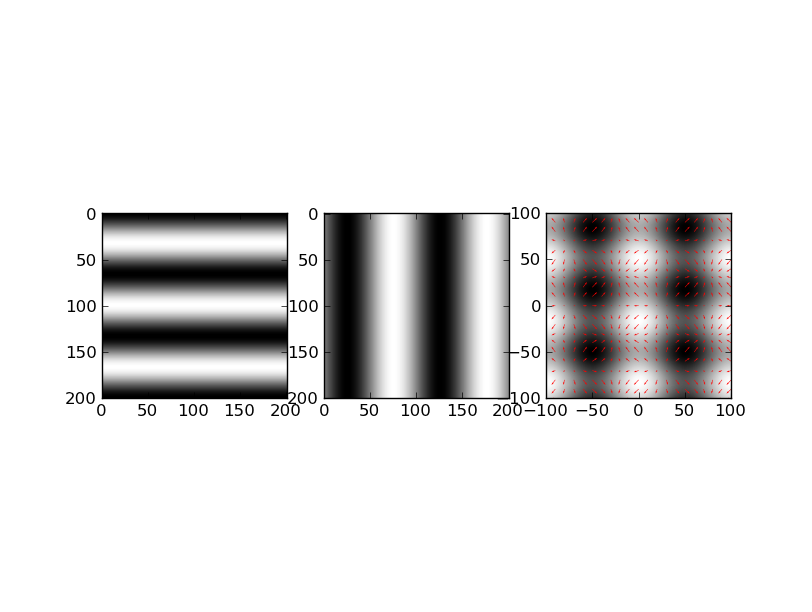
\includegraphics[scale=0.6]{quiver.png}
	\caption{Visualization of $f_x$, $f_y$ and a quiverplot of $f$}
\end{figure}

\section{Gaussian Convolution}

To perform a Gaussian convolution, we need to make a Gauss filter. To
do this, we use the Gaussian function. For this part of the exercise,
we use the 2 dimensional Gaussian function, which is:\\
\\
$\frac{1}{2\pi \sigma^2}e^{-\frac{x^2 + y^2}{s\sigma^2}}$\\
\\
To create the filter, we apply this to each $(x, y)$ in a grid of size
$(6s + 1)$ x $(6s + 1)$.\\
We can visualize this so-called \emph{kernel} in 3D. This gives us the
following image:
\begin{figure}[H]
	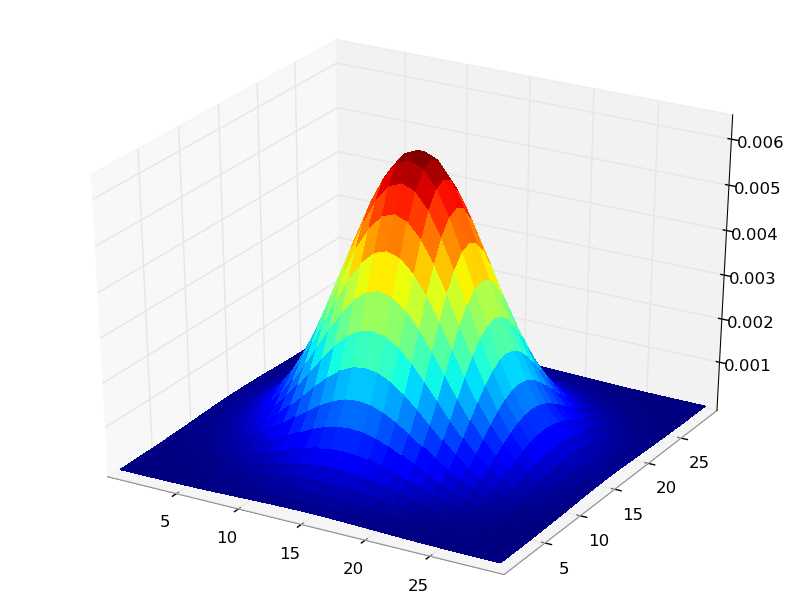
\includegraphics[scale=0.4]{kernel.png}
	\caption{Kernel of Gaussian filter for $s=5$}
\end{figure}

The complexity of this operation in $s$ is of order $\mathcal{O}(s^2)$.
This is because the program runs two loops, each over $(6s + 1)$. One of
these loops is inside the other, since we loop over the filter of size
$(6s + 1)$ x $(6s + 1)$. This means that we have a total of $(6s + 1) * 
(6s + 1)$ iterations, which leads to a total of $36s^2 + 12s + 1)$
iterations, which is of the order $\mathcal{O}(s^2)$.\\
This can also be seen in the following graph which plots the execution
time versus the size of $s$. This is obviously exponential:
\begin{figure}[H]
	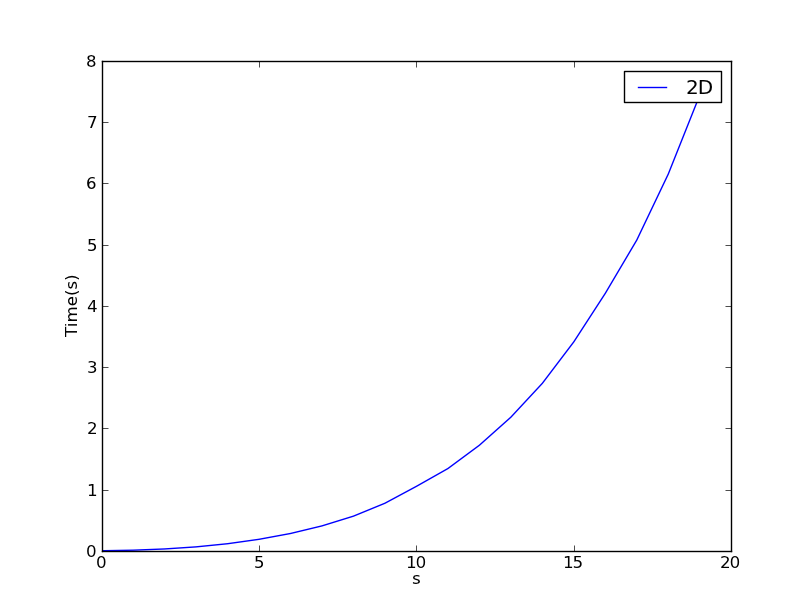
\includegraphics[scale=0.4]{2d.png}
	\caption{Two dimensional Gaussian convolution}
\end{figure}

\section{Separable Gaussian Convolution}

A performance increase for the Gaussian Convolution can be gained by
applying the convolution first in one direction and then in the
second. This way, we only have to calculate once in the x-direction and
once in the y-direction of the filter, instead of for each x and y.\\
That this is possible can be seen in the following proof:\\
\\
$\frac{\delta}{\delta x}\frac{\delta}{\delta y}G_{2D} 
= \frac{\delta}{\delta x}(\frac{\delta}{\delta x}(G_{1D}(x) * G_{1D}(y)) 
= \frac{\delta}{\delta x}(G_{1D}(x) * \frac{\delta}{\delta y}G_{1D}(y))
= \frac{\delta}{\delta x}G_{1D}(x) * \frac{\delta}{\delta y}G_{1D}(y)$\\
\\
This means that for each $s$ the order $\mathcal{O}(s)$. This is because
the Gaussian function has to be applied $n$ times per direction, with
$n = ceil(6s + 1)$. This means that the total times the Gaussian function
has to be applied is $2 * (6s + 1) = 12s + 2$. This is in the order 
$\mathcal{O}(s)$.\\
If we plot the timings, this can be seen as well, the line is a straight
line.
\begin{figure}[H]
	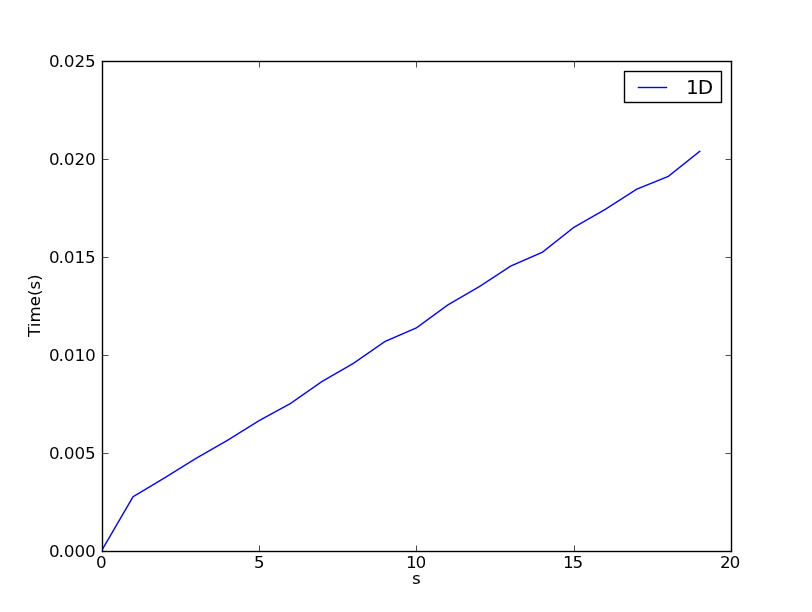
\includegraphics[scale=0.4]{1d.png}
	\caption{One-dimensional Gaussian convolution}
\end{figure}

\section{Gaussian Derivatives}

The Gaussian derivative of an image is the image that is obtained by
convolving the image with a derivative of the Gaussian function. To do this,
first we will need the first and second derivative of the one-dimensional
Gaussian function. These are as follows:\\
$f'(x) = \frac{1}{2\pi s^4} * (-xe^{-\frac{x^2}{2s^2}})$\\
$f''(x) = \frac{1}{2\pi s^6} * (-x^2 - s^2) * e^{-\frac{x^2}{2s^2}}$

We can apply these functions in different levels on the image, creating a
so-called `2-jet':
\begin{figure}[H]
	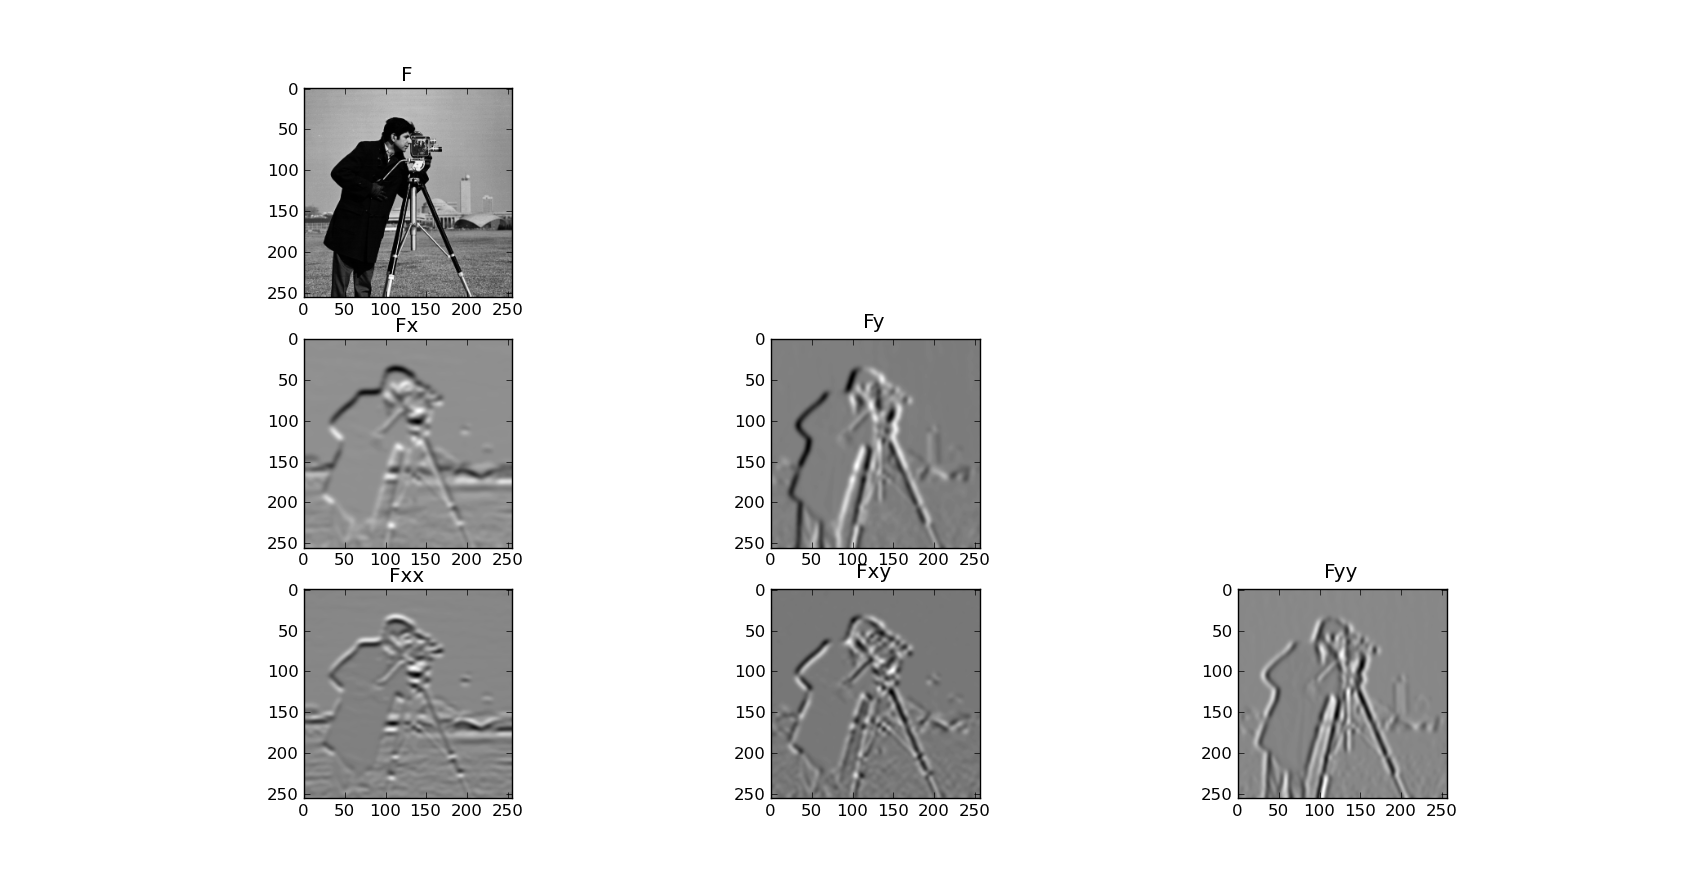
\includegraphics[scale=0.3]{jet.png}
	\caption{2-Jet}
\end{figure}

\section{Canny Edge Detector}

The final exercise was to implement the Canny Edge Detector. In the assignment we
were said to check in a 3x3 neighbourhood for both negative and positive sides on
either side of the pixel. However, this did not work properly for us. Instead, we
implemented the detector as described on 
\url{http://suraj.lums.edu.pk/~cs436a02/CannyImplementation.htm}, which includes
the use of a non-maximum suppression step, where you find the 'core' of a line by
checking the surrounding pixels in the direction that is perpendicular to the line,
and hystheresis thresholding, where you follow the line to see what points are noise
and what points are actually part of the line. This gives us the following result:\\

\begin{figure}[H]
	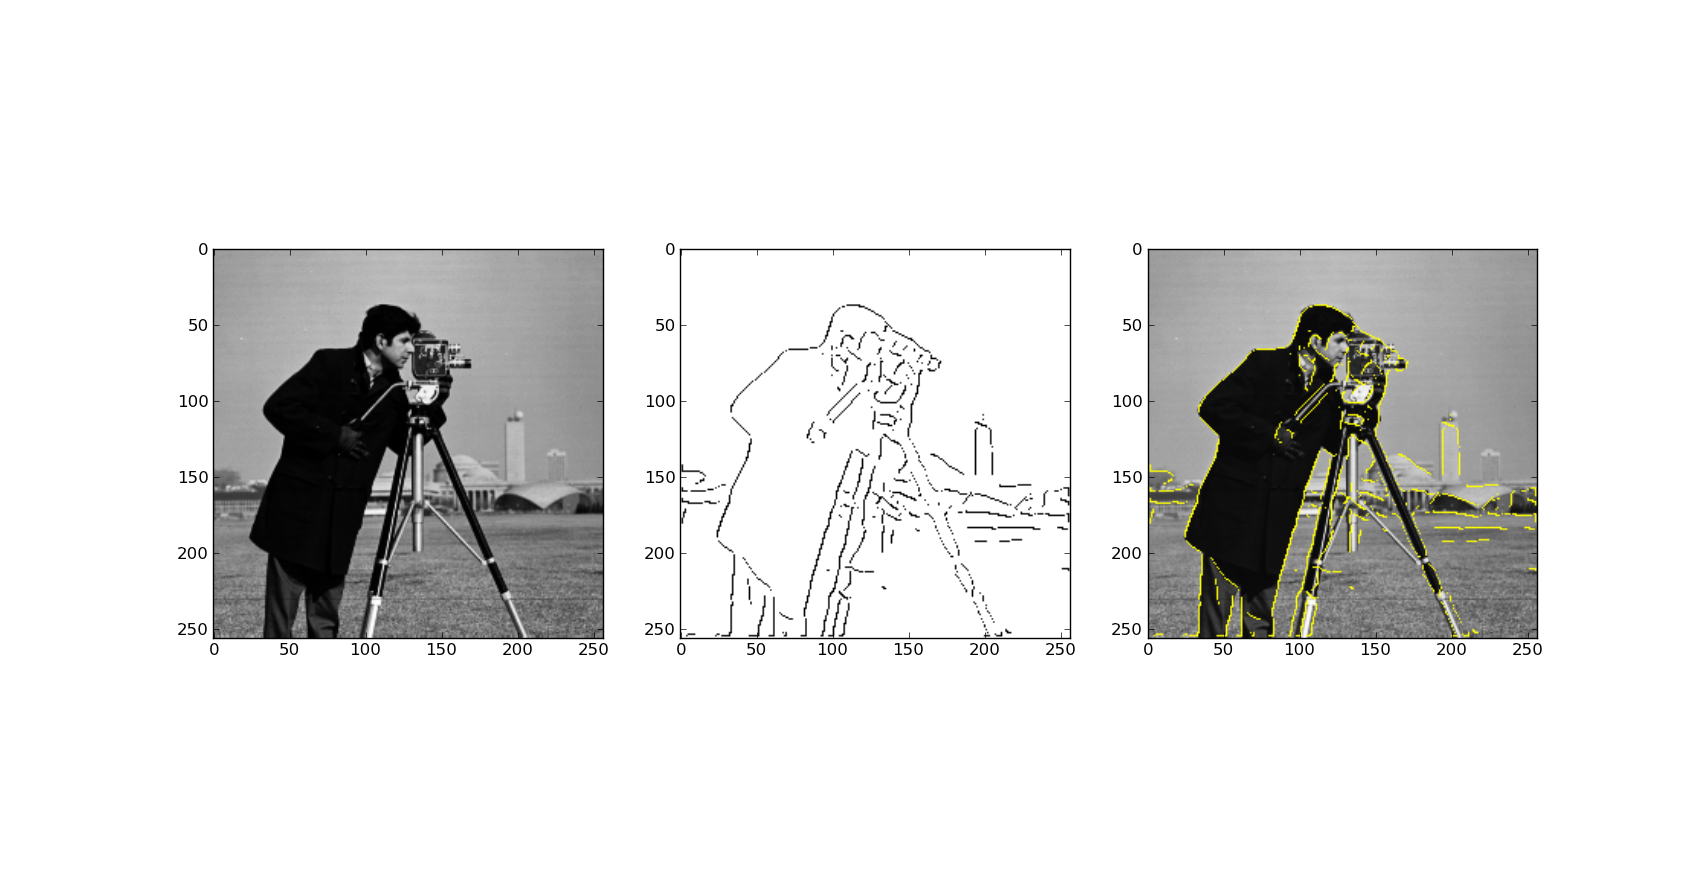
\includegraphics[scale=0.3]{canny.png}
	\caption{Canny Edge Detector}
\end{figure}

\end{document}